\chapter{TraMoS in the TESS era}\label{chap:tess}

With the end of the Kepler mission, thousands of possible exoplanets remain as candidates known as Kepler Objects of Interest (KOI). The Kepler Object of Interest Network (KOINet: \citep{vonEssen2018,Freuddenthal2018}) in the Northern hemisphere, is a network of ground-based telescopes performing photometric follow-up of KOIs to continue what Kepler left undone. The main goal of KOINet is to combine Kepler data with ground-based observations in order to confirm and characterize the masses of exoplanet candidates using TTVs.

It is crucial for TTV studies to continue the work of space missions from ground. It is unlike, only with space-based observations, to cover the interaction timescales to dynamically prove the TTV signal and the existence of possible companions, as in shown in Figure \ref{koinet}. In this figure, new data from ground-based telescopes were fundamental to confirm the TTV signal, and therefore to perform a proper characterization of the system.

\begin{figure}
\centering
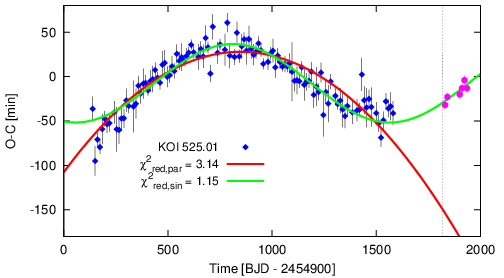
\includegraphics[width=0.8\columnwidth]{imagenes/koinet.png}
\caption{Observed minus calculated (O-C) diagram of the KOI-525b transit times, from the KOINet project. The observations from Kepler are in blue, and two different models were fitted on those data: an orbital decay model is in red, and a periodical TTV model is in green. If only Kepler data is considered, the two model could be plausible. The new ground-based observations (in pink) were essential to confirm the TTV nature of the system, discarding an orbital decay}
\label{koinet}
\end{figure}

The new space telescope Transiting Exoplanet Survey Satellite (TESS: \cite{Ricker2014}) is providing its first discoveries. The TESS observation plan divided in 13 sectors will challenge the confirmation process and characterization of possible exoplanets. During the $\sim27$ days of each sector, many candidates will not be observed enough time to confirm and characterize them. However, this special feature will provide a huge amount of new transit events of already known transiting exoplanets, specially for those with short-period. Combining the new TESS data with ground-base follow- up observations, many possible TTVs could be confirm or rule out. Moreover, \cite{Ballard2018} predicted that around 5\% of the planets discovered by TESS will exhibit measurable TTV signals, similar to Kepler’s results.

Between Sector 1 and Sector 13, TESS observed around 15\% of the stars with confirmed exoplanets but not all of them will produce a transit event within the 27 days of a sector duration (see Figure \ref{chap:tess}). Anyway, several complete light curves could be obtained and analyzed. TESS data are reduced by the Science Processing Operations Center (SPOC) and after being processed, they are archived in the Mikulski Archive for Space Telescopes (MAST) catalogue, where can be downloaded directly by anyone. 

\begin{figure}
\centering
\includegraphics[width=1.0\columnwidth]{imagenes/tess_match.pdf}
\caption{Match between all the stars with confirmed exoplanets and the TESS targets from Sector 1 to Sector 13. The empty red circles correspond to the star with confirmed exoplanets distributed by its position in the sky, while the filled red circles indicate if the exoplanet has an orbital period of less than 27 days, which is the duration of one TESS sector. The black cross indicates which star was already observed by TESS. However, this does not indicate that transit light curves will be provided for sure since the orbital period of the exoplanet needs to be taken into account. Thus, the first year mission of TESS will provide for sure transit data of the exoplanets with filled red circle and a black cross .}
\label{match_tess}
\end{figure}

Thus, for the currently and future stage of the TraMoS project, archival data - collected since 2008 - will be combined with the upcoming TESS data and new ground-based observations using one-meter class telescopes. The main goal of the project will remain the same: refine orbital and physical parameters of exoplanetary system and search for variations in the transit time, that could suggest the presence of additional small bodies in the system.  The KOINet project proved that ground-based follow-up are, in some cases, essential to complete a possible TTV signal, and therefore, to confirm or rule out variations in the transit time. During its first year of mission, TESS will supply with consecutive transit light curves from southern targets, specially from short-period planets, such as hot Jupiters. This special feature is fundamental to construct TTV curves and then, complete them from ground-based follow-up.

In the following subsections, I present a re-analysis of the TTV curves of the hot Jupiters: WASP-18b, WASP-19b and WASP-77Ab including new transit times from TESS: 45, 28, and 15 for WASP-18b, WASP-19b and WASP-77Ab respectively. In order to compute the transit time of each light curve, I used EXOFASTv2 but only to fit the transit time and the flux baseline. The remaining planetary parameters were fixed with the values from Tables \ref{wasp18}, \ref{tab:wasp19}, \ref{tab:wasp77}.

\section{WASP-18b}

The star WASP-18 was observed continuously during Sector 2 and 3 of the TESS mission, between August 22nd and October 18th, 2018. These observations provided 47 transits events of WASP-18b, but only 45 of them were complete transits, and therefore included into the TTV analysis. 

The new best linear fit for the period considering a total of 63 transit times is:

\begin{equation}
P = 0.941452232 \pm 2.7\times10^{-8} ~\rm days
\end{equation}

This value differs from the previous reported in Eq.~\ref{eq1_w18} by $0.016$ seconds, and the error was reduced to a third.

Figure \ref{wasp18_ttv} shows the extension of the TTV curve of WASP-18b considering the new data from TESS. Including these new transit times, the scatter from the linear ephemeris was reduced to 47 seconds. A possible second order fit of a hypothetical orbital decay, has a reduced chi squared of $\chi^{2}_{red}=0.35$, while the linear fit - which corresponds to the linear ephemeris - has $\chi^{2}_{red}=0.36$. Furthermore, as there is no strong evidence for an orbital decay in this system as proposed by \cite{Wilkins2017}, the simpler model should be chosen: the linear model.

Considering the lack of a clear sinusoidal TTV signal with even more transit time data, suggest that this exoplanet does not have a close-in companion in MMR. Moreover, the existence of a possible far-out companion is rejected by the lack of an additional signal in RV data. With this study, I can not discard the presence of any kind of companion of WASP-18b but if there is one, it should be small. 


\begin{figure}[h]
%\vspace{0.1cm}\hspace{0.2cm}
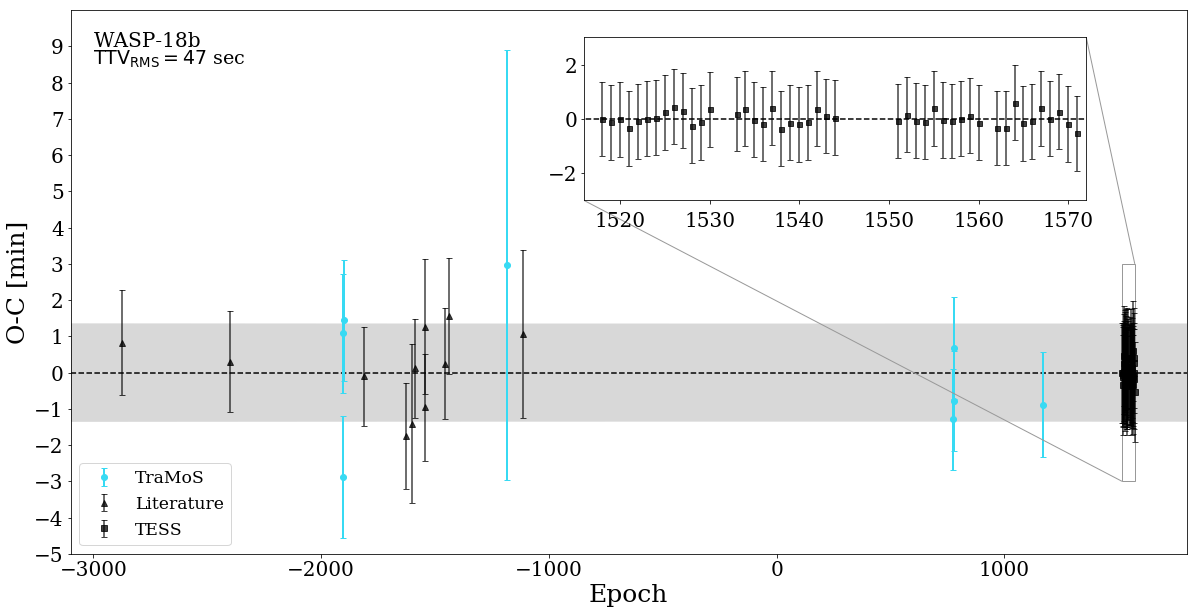
\includegraphics[width=1.0\textwidth]{imagenes/WASP18_TTV.pdf}
\caption{Observed minus calculated mid-transit times (TTV) for WASP-18b. The dashed black line corresponds to the proposed linear ephemeris, i.e. zero deviation from the predicted transit time  computed from our refined orbital period. For that, we considered 63 transit times from the TraMoS project (in light blue), published works and TESS (both in black). The grey area corresponds to the error propagation at $1\sigma$. The RMS scatter from the linear ephemeris is 47 seconds.}
\label{wasp18_ttv}
\end{figure}

\section{WASP-19b}

WASP-19 was observed during Sector 9 between February 28th and March 26th, 2019. During this time, 29 complete transit event were provided, and then considered to compute the new TTVs of WASP-19b show in Figure \ref{wasp19_ttv}. The new best fit for the orbital period P, considering a total of 88 transit times is:

\begin{equation}
P = 0.788838940 \pm 3.0\times10^{-8} ~\rm days
\end{equation}

The previous reported value in Eq.~\ref{eq1_wasp19} is $0.007$ seconds larger.

As in the case of WASP-18b, the TTV scatter of WASP-19b was reduced when including new transit times data from TESS to: $TTV_{RMS}=65~\rm seconds$. Again, a second order fit is not better that the linear one: $\chi^{2}_{red,lineal}= 0.65$ and $\chi^{2}_{red,cuad}= 0.64$. 

\begin{figure}[ht]
%\vspace{0.1cm}\hspace{0.2cm}
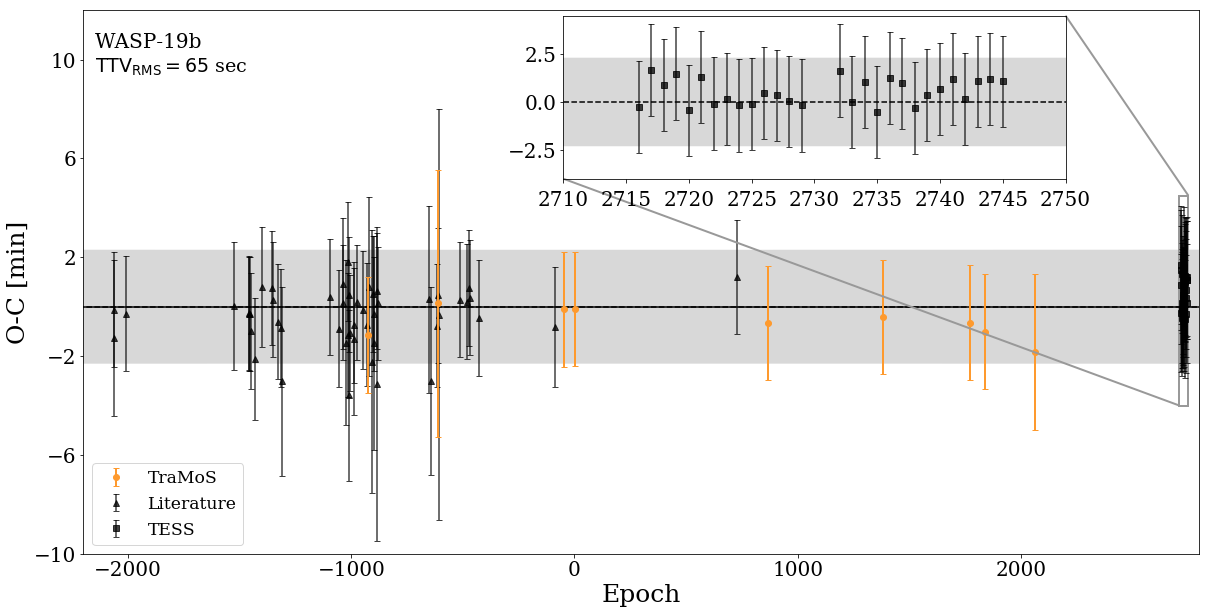
\includegraphics[width=1.0\textwidth]{imagenes/WASP19_TTV.pdf}
\caption{Observed minus calculated mid-transit times (TTV) for WASP-19b. The dashed black line corresponds to the proposed linear ephemeris, i.e. zero deviation from the predicted transit time  computed from our refined orbital period. For that, we considered 87 transit times from the TraMoS project (in light blue), published works and TESS (both in black). The grey area corresponds to the error propagation at $1\sigma$. The RMS scatter from the linear ephemeris is 65 seconds.}
\label{wasp19_ttv}
\end{figure}

\section{WASP-77Ab}

The third target presented in Cortés-Zuleta et al. 2019 (submitted), was observed in Sector 4 between October 18th and November 15th, 2018.  During this time, the planet transited its host star 17 times, but only 15 were complete light curves. From the previous study presented in this thesis, WASP-77Ab was the most interesting target, since its variation from the linear ephemeris was around  $121\,\rm seconds$.  After including the new transit times, the best linear fit for the orbital period is:

\begin{equation}
P = 1.36002866 \pm 1.7\times10^{-7} ~\rm days
\end{equation}

In Eq.~\ref{eq1_w77}, the value for the orbital period P is $0.01\,\rm seconds$ lower, and the scatter from the linear ephemeris was reduced to 86 seconds. The linear fit has a reduced chi squared of $\chi^2_{red}=1.03$, while a second degree polynomial has $\chi^2_{red}=0.72$. Anyway, the second order fit is highly dominated by the outlier transit time of epoch $229$ (see Figure \ref{wasp77_ttv}). After removing it, the reduced chi squared is  $\chi^2_{red}=0.37$. In all cases, the best fit correspond to the linear ephemeris.

As the previous two targets, extending the TTV curve of WASP-77Ab with transit times from TESS light curve supported the conclusion from the previous study: there is not a clear sinusoidal signal in the variations of the transit times, that could suggest a periodic TTV in WASP-77Ab. However, from the current work this target is the one with less transit time data, thus, follow-up observations would be required to confirm the no existence of close-in companions in MMR.


\begin{figure}[ht]
%\vspace{0.1cm}\hspace{0.2cm}
\includegraphics[width=1.0\textwidth]{imagenes/WASP77_TTV.pdf}
\caption{Observed minus calculated mid-transit times (TTV) for WASP-77Ab. The dashed black line corresponds to the proposed linear ephemeris, i.e. zero deviation from the predicted transit time  computed from our refined orbital period. For that, we considered 26 transit times from the TraMoS project (in light blue), published works and TESS (both in black). The grey area corresponds to the error propagation at $1\sigma$. The RMS scatter from the linear ephemeris is 86 seconds.}
\label{wasp77_ttv}
\end{figure}


%\section{WASP-36b}

%The exoplanet WASP-36b was selected as the